\chapter{Evaluation}
\label{chap:evaluation}

\section{Testing}

When developing an algorithm library for formal analysis of safety
critical systems it is vital to verify the correctness of the
implementation. Since the complexity of the code base makes formal
verification difficult we confined ourselves to rigorously testing the
functionalities provided by the library.

In this section, we summarize work presented in%
~\citep{TDK2015_Klenik_Marussy} that was performed to verify the
correctness of our implementation of the data structure, operations
framework and the stochastic analysis algorithms.

\subsection{Combinatorial testing}

As described in \cref{chap:operations} algorithms use the common
vector and matrix data structure to perform various operations. This
makes the used storage techniques transparent which in turn makes the
code base more concise, reusable and less prone to errors.

The most important requirement concerning the data structure and
operations is mathematical correctness regardless of the storage
technique and manner of execution (e.g.~parallel or sequential)
used. Considering the number of implementations for a given interface
and the previous requirement we used a simple unit testing design
pattern (also known as interface testing pattern) as the core building
block for the data structure testing \citep{myers2011art}.

The basic idea behind this pattern is to write unit tests for
interface operations without any knowledge about the concrete
implementation. Hiding implementation details can be achieved in a
number of ways. Some unit testing frameworks, such as \textsc{NUnit}%
~\citep{NUnit}, support the usage of generic test classes and running
them for multiple concrete types.

Since most of the time multiple instances of different types of
interface implementations are needed in a single unit test we choose a
more flexible approach for hiding implementation details. This
approach is based on class inheritance and abstract factory
methods. Whenever an instance if a given interface is needed, the
instantiation is delegated to an abstract factory method in the test
class.

\emph{Abstract test cases} were created to describe desired behaviors
of the operations. \emph{Concrete test cases} are derived from
abstract tests and contain calls to the data structure factory
methods. Thus, the behavior of any operation may be tested for all
possible data structure classes.

\subsubsection{Abstract tests}

Writing unit tests for valid parameter values is straightforward since
it is possible to cover multiple valid parameter ranges with a single
unit test. However testing for invalid parameter values requires some
care. There must only one invalid parameter per unit test lest one
error can obscure the others. This significantly increases the number
of unit tests. Therefore we aimed to gather every possible invalid
parameter range automatically.

We used Microsoft IntelliTest%
\footnote{formerly known as \textsc{Pex}~\citep{tillmann2008pex}}%
~\citep{IntelliTest}, which assists in automating white-box and unit
testing. IntelliTest automatically generates unit tests using
constraint satisfaction problem solving based on the source code of
the method under test. Using IntelliTest on our interface code
contract classes provided many invalid parameter values which were
used in abstract unit tests.

\subsubsection{Concrete tests}

Derived classes of abstract tests are created for every possible
combinations of data structure classes by implementing the abstract
factory method. Since the number of possible combinations is too large
to implement manually derived classes were generated with a Microsoft
Text Template Transformation Toolkit~(\textls{T4})~\citep{T4}
template.

Pairwise testing was used to decrease the number of generated tests
compared to full combinatorial testing of implementation
combinations. To generate the combinations for pairwise testing we
used the \textls{ACTS} tool \citep{borazjany2012combinatorial}.

As a result of this testing process more than $78\;000$ unit tests
were generated using full combinatorial testing (more than $18\;000$
with pairwise testing) which together with the behavior configuration
files serve as a quasi-formal specification for the expected behavior
of future and modified implementations (e.g.~performance
optimization).

Breaking changes in implementation should either be rejected or the
test suite and configuration files should be revised as specification
change. Every unit test was executed successfully for both sequential
and parallel operation implementations.

Concrete tests were executed with both configurations provided by the
operation framework as defaults, i.e.~parallel and sequential, to
ensure that computations are logically equivalent.

\subsection{Software redundancy based testing}

In addition to testing the data structure and operation
implementations, it is vital to test the correctness of higher level
algorithms used in the analysis workflow, e.g.\ the linear equation
solver and transient analysis algorithms.

Testing every implemented algorithm with unit tests would be
tremendous work that cannot be easily automated or maintained.
Moreover, every algorithm is used as part of a bigger workflow which
raises the question of compatibility of algorithms during an analysis.

As described in \cref{chap:overview:sec:our-workflow} for almost every
step of the workflow numerous algorithms are available.

\begin{obs}
  \label{obs:evaluation:reward-results}
  The result of a performance analysis (e.g.\ reward calculation) is
  mathematically independent of the used analysis workflow. It only
  depends on the possible behaviors of the system and the definition
  of the required performance measure. Two results calculated by two
  different analysis methods can only differ from each other due to the
  numerical properties of the algorithms.
\end{obs}  

Combining our fully configurable workflow with
\cref{obs:evaluation:reward-results} presents a new approach for
testing the algorithm implementations in a maintainable and almost
automatic manner. We can take advantage of the concept of software
redundancy commonly used in safety critical applications.

The main idea behind software redundancy is to perform a calculation
multiple times with usually fundamentally different algorithms
--~often developed by independent teams~-- thus minimizing the
possibility of common mode failures. After the calculations a voting
component examines whether every algorithm calculated the same
result. If that's not the case then one or more of the algorithms are
incorrect.

In this testing phase our analysis workflow is ran with a given
configuration and the calculated reward and sensitivity values are
saved. $588$ mathematically consistent configurations were generated
and executed on multiple benchmark models and case studies. The
maximum absolute difference of the calculated results was examined as
an error indicator.

\section{Measurements}

In this section we introduce the models used throughout the testing
and benchmarking phase and present results about the performance of
solver algorithms using the sparse matrix and block Kronecker
decomposition matrix forms.

Every model used for testing and measurement is publicly available at
\url{https://github.com/kris7t/stochastic-analysis} in a variety of
stochastic modeling formats.

\subsection{Models}
\label{sec:evaluation:models}

\subsubsection{Shared resource}

\begin{figure}
  \centering
  \begin{tikzpicture}
    \runningExamplePetriNet
  \end{tikzpicture}
  \caption{Stochastic Petri net for the \emph{SharedResource}
    model.}
  \label{fig:evaluation:model:sharedresource}
\end{figure}

Benchmark models were generated based on the Stochastic Petri Net
(\textls{SPN}) \emph{Shared\-Resource} model shown in
\cref{fig:evaluation:model:sharedresource}.

The model contains a number of clients competing for a central
resource ($p_S$). Each client may run a number of processes, which are
represented by token on $p_{C_i}$.

The model can be scaled by increasing the number of available shared
resources, the number of clients and the number of processes per
client. In \cref{ssec:evaulations:results}, $5$ clients were used and
the number of processes and shared resources were set to equal
values. In \cref{sec:evaulations:idrstab}, all parameters were swept
independently.

Symmetric~(Sym), slightly asymmetric~(Asym) and significantly
asymmetric~(Degen) versions of the model were created by assigning
transition rates. In the first case, all transition rates are equal to
$1$, while in the third case there are orders of magnitude of
difference between the transitions rates.

\subsubsection{KanBan}

The \textls{SPN} model of \emph{KanBan} (\textls{KB}) manufacturing
process \citep{ciardo2003logical} was used as another benchmark
model. The model was scaled by modifying the available resources at
each stage of the model resulting in an increase in the size of the
state space.

\subsubsection{Cloud performability}

The represents a \emph{Cloud} architecture \citep{ghosh2012scalable}
with physical and virtual machines serving incoming jobs using warm
and cold spare resources in case of increasing load. Some aspects of
the model in \citep{ghosh2012scalable} were modified because our
library currently does not support the Generalized Stochastic Petri
Net (\textls{GPSN}) formalism.

\subsection{Results}
\label{ssec:evaulations:results}

\begin{table}
  \caption{Operation configurations and algorithms used in the benchmarks.}
  \centering
  \begin{tabular}{@{}llll@{}}
    \toprule
    Analysis task & Operation config. & Solver & Inner solver \\
    \midrule
    Steady-state & Parallel & Gauss--Seidel & $-$ \\
    & & \textls{BiCGSTAB} & $-$ \\[1ex]
    & Sequential & Group Gauss--Seidel & \textls{BiCGSTAB} \\
    & & Group Gauss--Seidel & Jacobi \\[1ex]
    Transient & Parallel & Uniformization & $-$ \\
    \bottomrule
  \end{tabular}
  \label{tab:evaluation:algorithms}
\end{table}

\begin{table}
  \caption{Selected benchmark results (adapted from~\citep{TDK2015_Klenik_Marussy}).}
  \centering{\small
  \begin{tabular}{@{}lrllrr@{}}
    \toprule
    \multicolumn{1}{@{}c}{Model} & \multicolumn{1}{c}{States} &
    \multicolumn{1}{c}{Generator} & \multicolumn{1}{c}{Algorithm} &
    \multicolumn{1}{c}{Memory} & \multicolumn{1}{c@{}}{Time} \\
    \midrule
    SR-Sym-7 & $10\,775\,710$
    & Sparse & Uniformization & $3\,120$~MiB & $279$~s \\
    & & & \textls{BiCGSTAB} & $3\,450$~MiB & $236$~s \\
    & & \textls{BK} & Uniformization & $650$~MiB & $222$~s \\
    & & & \textls{BiCGSTAB} & $815$~MiB & $162$~s \\

    SR-Asym-7 & $10\,775\,710$
    & Sparse & Uniformization & $3\,116$~MiB & $316$~s \\
    & & & \textls{BiCGSTAB} & $3\,450$~MiB & $236$~s \\
    & & \textls{BK} & \textls{BiCGSTAB} & $812$~MiB & $373$~s \\

    SR-Degen-7 & $10\,775\,710$
    & Sparse & \textls{BiCGSTAB} & \multicolumn{2}{c@{}}{Breakdown} \\
    & & BK & Group \textls{GS} / Jacobi & \multicolumn{2}{c@{}}{No convergence} \\
    
    SR-Sym-9 & $81\,466\,099$
    & Sparse & \textls{BiCGSTAB} & $25\,564$~MiB & $2\,542$~s \\

    SR-Asym-9 & $81\,466\,099$
    & Sparse & \textls{BiCGSTAB} & \multicolumn{2}{c@{}}{Oscillation} \\
    & & \textls{BK} & Group \textls{GS} / Jacobi & $2\,388$~MiB & $9\,402$~s \\
    
    Cloud-3-2 & $20\,047\,500$
    & Sparse & \textls{BiCGSTAB} & \multicolumn{2}{c@{}}{Out of memory} \\
    & & BK & \textls{BiCGSTAB} & \multicolumn{2}{c@{}}{Breakdown} \\
    & & & Group \textls{GS} / Jacobi & $684$~MiB & $3\,379$~s \\
    
    KanBan-5 & $2\,546\,432$
    & Sparse & Uniformization & $833$~MiB & $54$~s \\
    & & & \textls{BiCGSTAB} & $911$~MiB & $92$~s \\
    & & BK & Uniformization & $360$~MiB & $70$~s \\
    & & & \textls{BiCGSTAB} & $392$~MiB & $124$~s \\

    KanBan-7 & $41\,644\,800$
    & Sparse & Uniformization & $12\,471$~MiB & $909$~s \\
    & & BK & Uniformization & $6\,253$~MiB & $1\,135$~s \\
    \bottomrule
  \end{tabular}}
  \label{tab:evaluation:results}
\end{table}

Benchmarks on large models were performed with the analysis
configurations shown in \cref{tab:evaluation:algorithms}. Each
analysis configuration was run with both sparse and block Kronecker
generator matrices. 19 models were created by scaling the models
described in \cref{sec:evaluation:models}.

Execution time was limited to 1~hour and the maximum memory allocation
was limited to 32~GiB. As runs for scaled versions of models were
omitted if the analysis was terminated due to limit crossing for a
smaller model, only 152 runs were performed in total. 81 runs exited
after successful calculation of a result. Selected results are shown
in \cref{tab:evaluation:results}.

\Cref{fig:evaluation:bicgstab-time,fig:evaluation:bicgstab-memory}
illustrate the state space size dependence of the behavior of the
\textls{BiCGSTAB} linear equation solver.
\Cref{fig:evaluation:uniformization-time,fig:evaluation:uniformization-memory}
illustrate the state space size dependence of the uniformization
transient analysis algorithm.

\begin{figure}
  \centering
  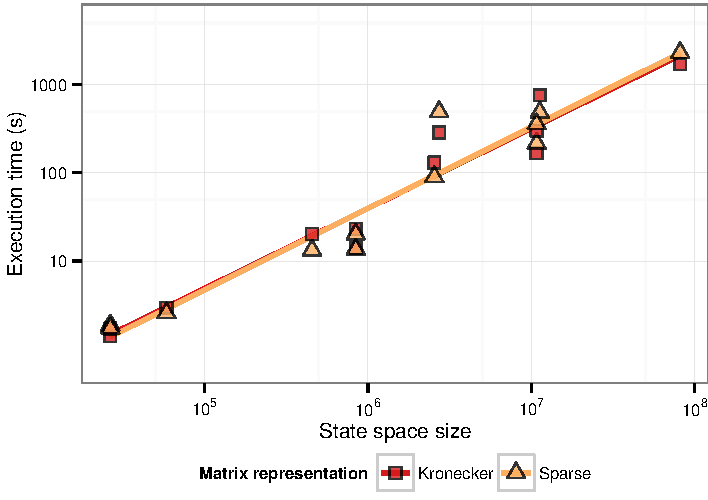
\includegraphics{figures/Bicgstab_matrix_time}
  \caption{Execution times of steady-state analysis with the
    \textls{BiCGSTAB} solver.}
  \label{fig:evaluation:bicgstab-time}
\end{figure}

\begin{figure}
  \centering
  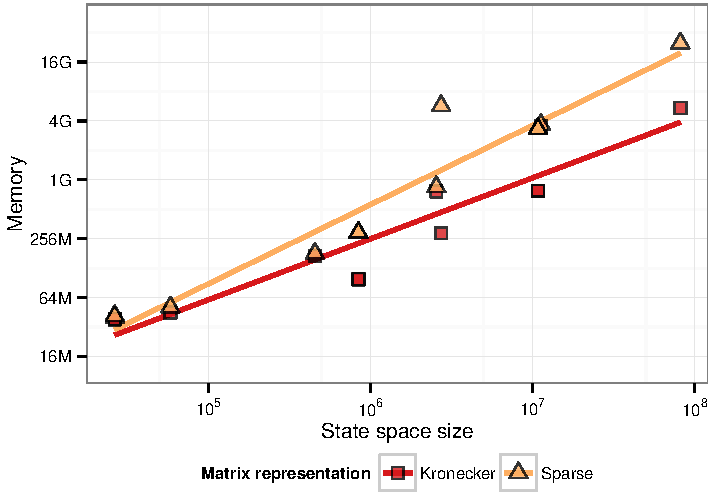
\includegraphics{figures/Bicgstab_matrix_memory}
  \caption{Memory consumption of steady-state analysis with the
    \textls{BiCGSTAB} solver.}
  \label{fig:evaluation:bicgstab-memory}
\end{figure}

\begin{figure}
  \centering
  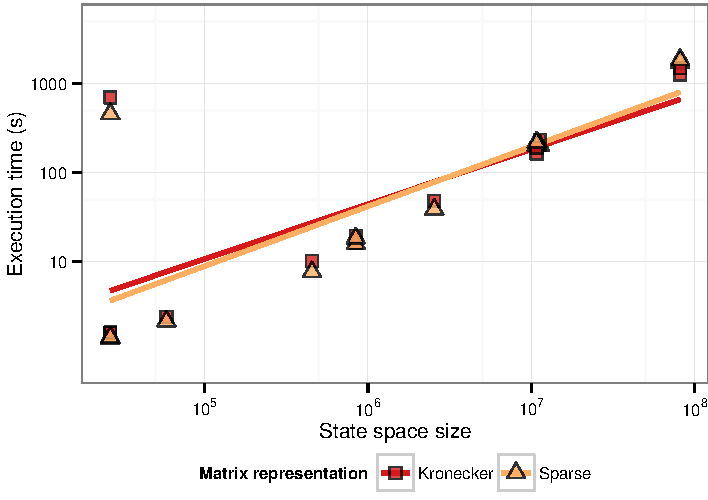
\includegraphics{figures/Uniformization_matrix_time}
  \caption{Execution times of transient analysis with
    uniformization.}
  \label{fig:evaluation:uniformization-time}
\end{figure}

\begin{figure}
  \centering
  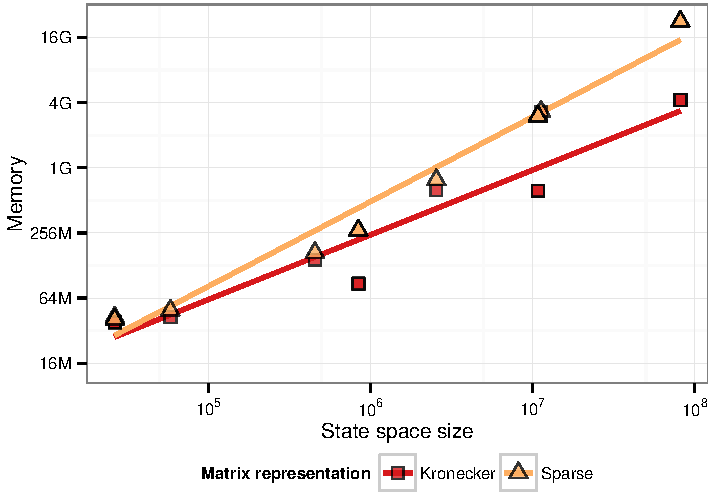
\includegraphics{figures/Uniformization_matrix_memory}
  \caption{Memory consumption of transient analysis with
    uniformization.}
  \label{fig:evaluation:uniformization-memory}
\end{figure}

As expected the storage requirements of block Kronecker generator
matrices are almost an order of magnitude smaller than those of sparse
matrices.

For models with less than a few millions states the sparse form of the
generator matrix outperforms the block Kronecker form. However, for
models with considerably bigger state space sizes the block Kronecker
form reduces both the execution time and memory requirements of the
analysis compared to the sparse form, which is also apparent in
\cref{fig:evaluation:bicgstab-time,fig:evaluation:bicgstab-memory,%
  fig:evaluation:uniformization-time,fig:evaluation:uniformization-memory}.
A possible reason for this phenomenon is inefficient \textls{CPU}
memory cache usage of the sparse storage.

We can conclude that while block Kronecker generator matrices stored
as expression trees are significantly more complicated than sparse
storage, the configurable operations framework managed to perform the
matrix multiplications efficiently for both small and large model
state spaces.

For models with similar transition rates the BiCGSTAB algorithm was
found the most effective steady-state solution method for both sparse
and block Kronecker matrices.

Slower, but more memory efficient algorithms, such as Gauss-Seidel
iteration and Jacobi iteration, often diverged with the sparse matrix
form while converged using the block Kronecker form. This is due to
different state orderings in the different matrix representations.

For irregular models with transition rates of orders of magnitude
difference it is possible that \textls{BiCGSTAB} will not converge
while other algorithms yield a solution, albeit only after many
iterations.

In transient analysis, orders of magnitude differences in transition
rates lead to highly \emph{stiff} models. High stiffness increases the
number of iterations performed by uniformization significantly. In
\cref{fig:evaluation:uniformization-time}, the stiff
\emph{\textls{SR}-Degen-3} model appears as an outlier with nearly
500~s execution time despite having only $26\,464$ states. Transient
analysis of larger versions of the \emph{\textls{SR}-Degen} did not
finish withing the time limit.

\section{The convergence of \textls[30]{IDRSTAB}}
\label{sec:evaulations:idrstab}

To study the convergence properties of
\textls{IDR}($s$)\textls{STAB}($\ell$), we created several scaled
versions of the \emph{SharedResource-Sym} model by varying the the
number of available shared resources, the number of clients and the
number processes per client between $1$ and $5$. This allowed
observing the behavior of the solver with a variety of matrix
sizes. In all problems sparse matrix storage was selected due to the
relatively small size of the state space.

\textls{IDR}($s$)\textls{STAB}($\ell$) was executed on the
steady-state linear equations arising from the generated stochastic
models with parameter settings $s = 1, 2, 4, 8$ and $\ell = 1, 2, 4,
8$. Note that the case $s = \ell = 1$ is mathematically equivalent to
\textls{BiCGSTAB}, albeit with worse numerical properties in
finite-precision arithmetic.

Due to the random initialization of the shadow Krylov subspace (see
\vref{alg:algorithms:idrstab:idrstab}) each experiment was repeated
with five different random seeds. Therefore $10\,000$ runs were
performed in total.

The histogram of the observed behaviors of
\textls{IDR}($s$)\textls{STAB}($\ell$) is shown in
\cref{fig:evaluation:idrstab:histogram}. Each histogram shows the
observations for a particular $(s, \ell)$ parameter setting. As the
cases $s = 4$ and $\ell = 4$ show performance very similar to $s = 8$
and $\ell = 8$, therefore they were omitted in the interest of
reducing clutter.

\begin{itemize}
\item ``Success'' refers termination of the algorithm with a solution
within $200$ iterations.
\item ``Breakdown'' refers to calculations that resulted in a singular
$\largesigma$ matrix and therefore terminated.
\item ``Divergence'' yielded residual norms increasing to the limit of
double-precision floating point.
\item ``No result'' cases failed to produce a solution in $200$
iterations, but did not otherwise fail.
\end{itemize}

In addition, the first $50$ iterations of trajectories from $5\,625$
short experiments are summarized in
\cref{fig:evaluation:idrstab:traj}. The trajectories are grouped by
$(s, \ell)$ parameters and state space size.

It is apparent that only $s = 1$ cases managed to decrease residual
norm and only $\ell = 1$ lead to reliable decrease of residual norm
over iterations for larger state spaces.

For the other parameter settings, successful exit from the iteration
happened only due to our modifications to
\textls{IDR}($s$)\textls{STAB}($\ell$) introduced in
\vref{alg:algorithms:idrstab:idrstab,alg:algorithms:idrstab:idr,%
  alg:algorithms:idrstab:gmres}. However, stability of convergence is
still lacking, as our proposed modifications are unable to handle
singular or nearly singular $\largesigma$ matrices that arise when
\textls{IDR}($s$)\textls{STAB}($\ell$) is applied to steady-state
analysis of \CTMC\ models.

Settings with $\ell > s$ tend to result in rapid divergence of the
residual to infinity, while $\ell \le s$ often breaks down or
oscillates.

Surprisingly, breakdowns occur even if $s = \ell = 1$, i.e.~if
\textls{BiCGSTAB} mode is used. Before breakdown, the residual norm is
approximately $6 \cdot 10^{-7}$. This number is probably the limit to
the accuracy of the \textls{IDR}($s$)\textls{STAB}($\ell$) formulation
of \textls{BiCGSTAB}, as the original \textls{BiCGSTAB} algorithm
utilizes a more stable residual update strategy.

\begin{figurepage}
  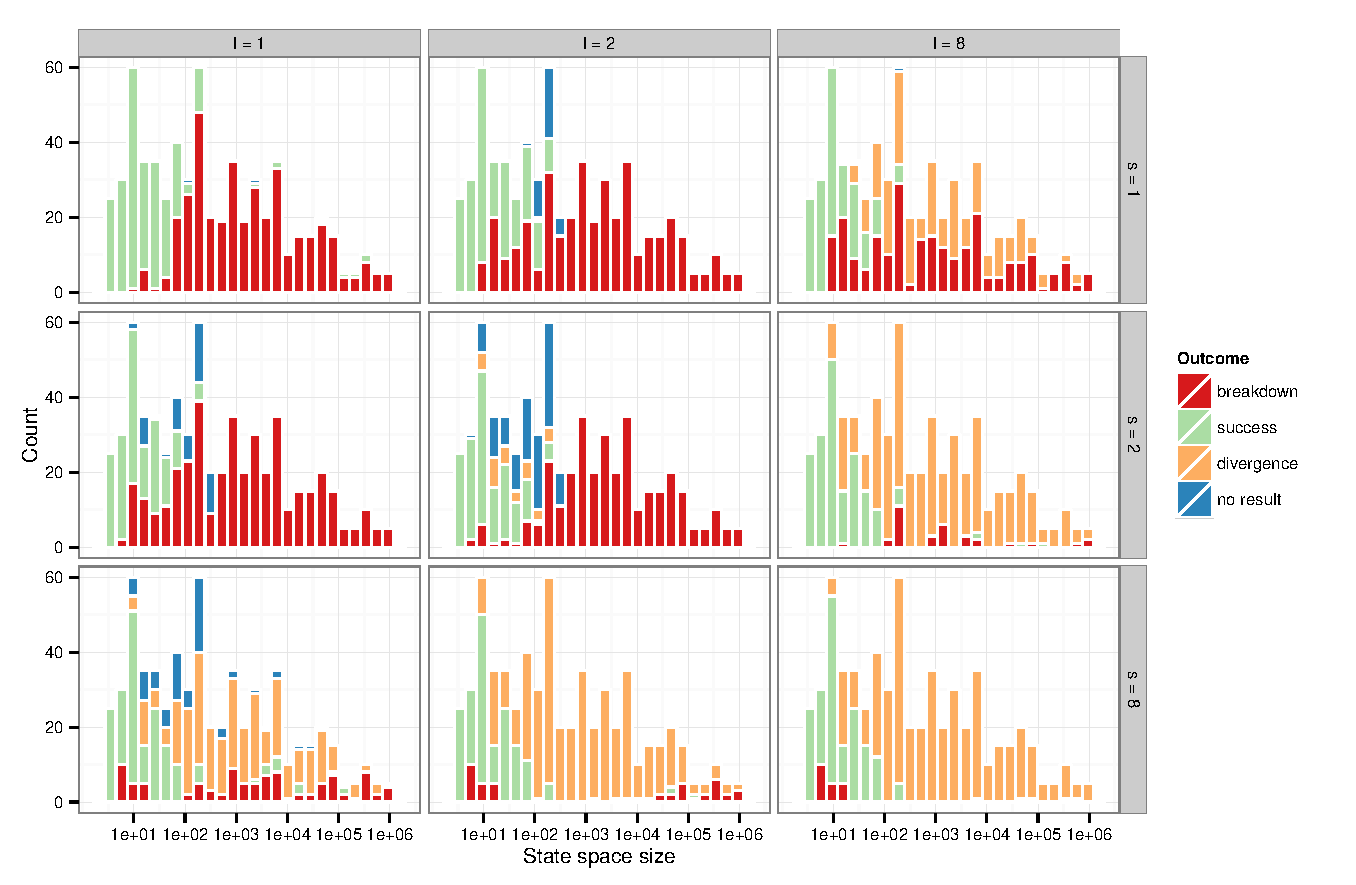
\includegraphics{figures/idrstab_histograms}
  \captionof{figure}{Histogram of observed behaviors of
    \textls{IDR}($s$)\textls{STAB}($\ell$).}
  \label{fig:evaluation:idrstab:histogram}
\end{figurepage}

\begin{figurepage}
  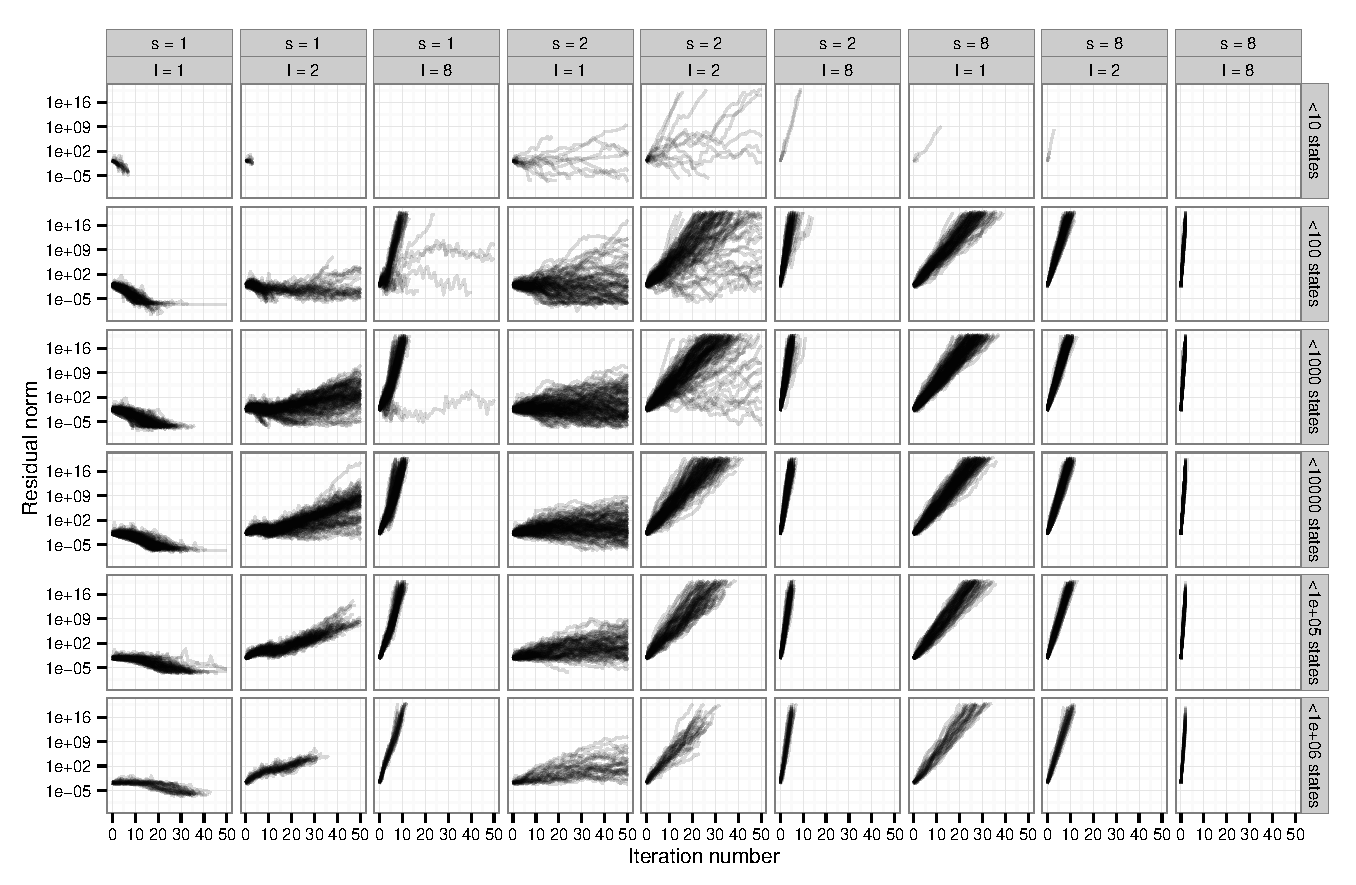
\includegraphics{figures/idrstab_convergence}
  \captionof{figure}{Convergence histories observed in various runs of
    \textls{IDR}($s$)\textls{STAB}($\ell$).}
  \label{fig:evaluation:idrstab:traj}
\end{figurepage}
